\documentclass[a4paper]{article}
\usepackage[utf8]{inputenc}
\usepackage{wrapfig}
\usepackage{caption}
\usepackage{graphicx}
\usepackage{geometry}
\usepackage{float}
 \geometry{
 a4paper,
 total={210mm,297mm},
 left=20mm,
 right=20mm,
 top=20mm,
 bottom=20mm,
 }


\pdfinfo{
  /Title    (Building Serious Games - Design4Health)
  /Author   (Ralf Nieuwenhuizen, David Prihoda, Ismini Psychoula, Arnold Schutter, Shen Shuheng)
  /Creator  (Ralf Nieuwenhuizen, David Prihoda, Ismini Psychoula, Arnold Schutter, Shen Shuheng)
  /Producer (Ralf Nieuwenhuizen, David Prihoda, Ismini Psychoula, Arnold Schutter, Shen Shuheng)
  /Subject  (Building Serious Games)
}

%Game technical report (no more than 8-10 pages)
%- describe and justify each of the main technical choices made in the prototype (including engine,
%libraries used, class structure, special-purpose algorithms, effects, user interaction, GUI, …)
%- what will be the main technical challenges for further developing the final game ?
%- (technical) recommendations and warnings; what did you try but failed? why ?

\title{Building Serious Games: Technical Report}
\author{
	R. Nieuwenhuizen \and
    D. Prihoda  \and
	I. Psychoula \and
	A.S.C. Schutter \and
	S. Shen
 }
\date{January 2015}

\begin{document}



\maketitle
\begin{abstract}
This report concerns the development of PhysioFun, a mobile phone game designed to encourage the users to exercise regularly. The software is based on Phonegap, a free and open source framework that allows the creation of mobile apps using standardized web APIs. 

The idea for the application originated from the project specifications set to us by Design4Health, a company that aims to ``apply user-centered design tools and methods to the field of healthcare, through a careful study of digital touch-points, behavioral science and a combination of digital and physical products to shape a new and better healthcare experience.''

It has been identified from the start that the software will be in a prototype stage upon submission, and it has only been tested with an Emulator and Android smartphones.
\end{abstract}

\renewcommand{\abstractname}{Acknowledgements}
\begin{abstract}
We would like to take the opportunity to thank our instructor Professor Bidarra and our mentors Mr. Dukalski and Mr. Ringard for their valuable guidance, stimulating suggestions and encouragement that helped us complete this project. We also would like to thank Mr. Barlage for the view on the exercises from the perspective of physiotherapy. 
\end{abstract}

\section{Introduction}
Nowadays, people are getting more and more stuck behind their desks or on the couch, which is the cause for many diseases. Physiofun is a mobile phone game designed to encourage the users to exercise regularly. The user will try to develop a farm in space, by completing real life exercises.\\
\\
The idea for the application originated from the project specifications set to us by Design4Health, a company that aims to ``apply user-centered design tools and methods to the field of healthcare. Through a careful study of digital touch-points, behavioral science and a combination of digital and physical products to shape a new and better healthcare experience.''\\
\\
The report will start off explaining the various design decisions we have made, and why we have made them. After that, the technologies used will be explained, followed by the game structure along with all the components in the game. Next there will be a part about the user interface, followed by a section about the sensors used to measure the exercises. The report will conclude with challenges we had during the development, and technical recommendations towards a real serious game, which is ready for the market, you can regard this as a ``wishlist''.

\section{Decisions}
This section provides more insight to our main choices for the project and our decision making process.
\\\\
One of the first things we had to think about was a way to incorporate our software with sensors since it was one of the goals of our project. 
\\\\
At the very start of the project we to make a decision if we would make the game for a computer or for a mobile device. Clearly we chose for a mobile game, the reason is that the devices already have incorporated sensors we want to use. Another decision we had to make is if our game would be played in iOS devices, Android devices or Windows phone. We decided to use the Phonegap framework since it would allow as to make the application available to all the above operating systems. 
\\\\
Another reason we chose for PhoneGap was that it seemed to be the most convenient way to develop an Android game. Most of us had more knowledge of web languages and less of other languages. PhoneGap seemed an easy tool to convert web pages to a native Android app. 
\\\\
Another decision was about the way to develop the graphics. Who chose not to use for 3D graphics with for example Blender because of the time and size constraints as it would make the size of the application much larger. It also would take much longer to design them. Instead we opted for 2D graphics and isometric tiles that would give our application the illusion of a third dimension.


\section{Technologies Used}
\subsection{PhoneGap}

PhoneGap is an open source framework for quickly building cross-platform mobile apps using HTML5, JavaScript and CSS. It is a convenient way to develop an Android game. It also gives the possibility to eventually extend to iOS to enlarge the target audience.

\subsection{HTML 5}

HTML5 is a core technology markup language of the Internet used for structuring and presenting content for the World Wide Web. It includes detailed processing models to encourage more interoperable implementations; it extends, improves and rationalises the markup available for documents, and introduces markup and application programming interfaces (APIs) for complex web applications [6]. For the same reasons, HTML5 is also a potential candidate for cross-platform mobile applications. Many features of HTML5 have been built with the consideration of being able to run on low-powered devices such as smartphones and tablets. We have chosen for HTML 5 because it is encouraged to use that for web-based games.

 \subsection{Closure}

The Closure Library is a JavaScript library, written specifically to take advantage of the Closure Compiler, based on a modular architecture. It provides cross-browser functions for DOM manipulations and events, Ajax and JSON, as well as more high-level objects such as User Interface widgets and Controls.

The Closure Library is a broad, well-tested, modular, and cross-browser JavaScript library. You can pull just what you need from a large set of reusable UI widgets and controls, and from lower-level utilities for DOM manipulation, server communication, animation, data structures, unit testing, rich-text editing, and more.
The Closure Library is server-agnostic, and is intended for use with the Closure Compiler.
Moreover, LimeJS uses Closure. 

\subsection{Closure compiler}
The Closure Compiler is a tool for making JavaScript download and run faster. It is a true compiler for JavaScript. Instead of compiling from a source language to machine code, it compiles from JavaScript to better JavaScript. It parses your JavaScript, analyzes it, removes dead code and rewrites and minimizes what's left. It also checks syntax, variable references, and types, and warns about common JavaScript pitfalls.

\subsection{LimeJS}
\label{subsec:limejs}

LimeJS is a HTML5 game framework for building fast, native-experience games for all modern touchscreens and 
desktop browsers.
LimeJS looks like another great entry into the HTML5 gaming space.  It is based on the Google Closure library, and supports rendering to both the DOM and to the HTML5 Canvas element
\\\\
We have chosen for LimeJS because it is a well-known game creation platform for the web. It provides fast and simple rendering a has proven to be a great framework for us.

\subsection{Box2d}

Box2DJS is a JavaScript port of Box2D Physics Engine.
This is a clone of a box2d JavaScript engine which is a clone of the box2d C++ library.
PixelLab modified the library to use Google's Closure JavaScript Compiler for great compression--with the added benefit of compile-time checking.
\\\\
The use of Box2d is required by the LimeJS library.


\subsection{Cordova plugins}
\label{subsec:cordova-plugins}

\begin{itemize}
  \item \textbf{org.apache.cordova.device}
  This plugin defines a global device object, which describes the device's hardware and software. Although the object is in the global scope, it     is not available until after the device ready event.
  
  \item \textbf{org.apache.cordova.device-motion}
    This plugin provides access to the device's accelerometer. The accelerometer is a motion sensor that detects the change (delta) in movement        relative to the current device orientation, in three dimensions along the x, y, and z axis.
  \item \textbf{ org.apache.cordova.media}
    This plugin provides the ability to record and play back audio files on a device.

\end{itemize}





\section{Code structure}
The source code of the project is divided into two parts, the actual game, and the part to make it run on Android. Both parts will be explained in the next paragraphs.

\subsection{Android code}
The outer structure of the source code is defined by the rules of Java, PhoneGap (Cordova), and Android. Here are the Android manifest and all the plugins needed for the game to run on the phone. More about these plugins can be read in paragraph~\ref{subsec:cordova-plugins}

\subsection{Game code}
Inside the assets folder is where the game is located. The structure of the game is defined by LimeJS.
LimeJS lets the user make an interface really fast and easy. You can just define shapes and buttons, customize them and put them on the screen. The game is composed of two types of components, objects and scenes, and also there are the images and sounds. All of these will be explained below. More on LimeJS can be read in paragraph~\ref{subsec:limejs}

\subsubsection{Objects}
Object contain information of the different game components. Example are exercise, items, crops, livestock, body and challenge. Each object can have methods assigned to it. For example, a challenge has methods to check whether all required items are available, and whether all exercises have been completed. It might be worth mentioning that there is also a separate settings file, where most of the major parameters for the gameplay and the user interface can be set. One of these settings is testing, which speeds up the game, and enables some shortcuts when set to true.

\subsubsection{Scenes}
At first, we used the LimeJS director for all of the screens, but it turned out that this way you could not click outside of the focused layer to click the menu buttons, so it was decided to change the structure a bit. Now, layers are simple pushed on top of the other screen, allowing the user to easily switch between each screen. All of these screen have their own file.

\subsubsection{Images}
The images are also divided into several folders. The crops and livestock for example have their own folders. Each exercise also has a separate folder, so the looping animation can be created easily.

\subsubsection{Sounds}
The sounds are located both in the game folder and the root folder, because Android/PhoneGap could not reach the sounds when they were in the game folder. The other way around, when testing the game in the browser, as was done, the sounds had to be in the game folder.

\section{User Interface}
The user interface has undergone extensive testing. Based on the test results the interface is changed multiple time to make it more intuitive. 

\subsection{Design}
The graphics were done in Adobe Illustrator and finalized in Adobe Photoshop. We decided for cartoon-style design because of its ease of drawing, ease of implementation and high creativity potential.

\subsection{Map}
To show the farm on the map, we decided for the isometric view. Compared to a regular rectangular view, it is much more visually appealing and relates to the story -- a birds eye view. Compared to a fully 3D approach, it is an order of magnitude easier to implement, and also provides significantly higher frame rates on a smartphone. By stacking tiles with the ZigZag algorithm, we create a fake 3D perspective.

\subsection{Sounds}
Sound were used to pull the player into the game. From our testing sessions we gathered that players mostly appreciate music and sounds, but they require a way to disable them. Therefore we introduced the settings window, where sounds and music can be disabled.

\subsection{Clickable objects}

To make it more clear that a certain crop or livestock is ready and needs action, it is now glowing. This drags the immediate attention of the user.

Moreover, we increased the size of buttons significantly compared to the first playable, to decrease the time the user has to spend positioning his finger on the screen. The drawback of this action was that we had to create additional screens because the display got too cluttered.

\subsection{Daily tasks}
Daily tasks are implemented to create more effect in the normal life of the user. The game has been extended and shows the uncle on the farm. The uncle provides the user with daily tasks. This seemed to be a convenient way to show more information.

\subsection{Introduction}
At the very start it was not clear what the buttons at the bottom of the screen were used for. We decided to create an introductional session to show all the features of the game in a playful way. After some tests it seemed that the introduction was obtrusive and enforcing the user too much. This has been improved by only giving a brief introduction, followed by a list of tasks which gives the freedom to the user to explore the game on his own.

\section{Sensors}
The Android Phone has a three direction accelerometer sensor that reads the change in speed along three axis ($x$, $y$, and $z$). 
Programs using the accelerometer read this information to give the phones orientation in space or the phones change in speed and direction. 
\\\\
In order to read this information an Acceleration object is populated and returned by any of the API's Accelerometer methods. Acceleration values include the effect of gravity ($9.81 m/s^{2}$), so that when a device lies flat and facing up, $x$, $y$, and $z$ values returned should be $0$, $0$, and $9.81$




\subsubsection{Exercise Algorithm}



\begin{figure}[H]
	\centering
		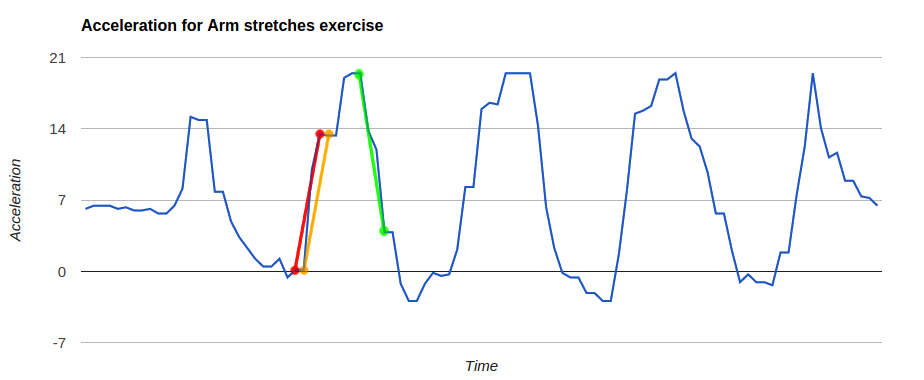
\includegraphics[width=0.80\textwidth]{images/Armstretch.png}
	\caption{Acceleration in the Y axis during the Arm Stretch exercise. The periodicity of exercises we have used provides an advantage when counting the number of finished repetitions. \textit{Up-steps} are marked in red and yellow, \textit{down-step} is marked in green.}
	\label{fig:acceleration1}
\end{figure}

Our final algorithm works by finding \textit{up-steps} and \textit{down-steps} in the acceleration values. An \textit{up-step} is defined at points where the difference in acceleration over $s$ last samples changed more than threshold $T$. A \textit{down-step} is defined at points with change larger than $-T$. 

The number of repetitions is then increased each time an \textit{up-step} appears, then a \textit{down-step} has to occur before the next repetition can be added. To counter impulsive noise, in the final version of the algorithm, we require two \textit{up-steps} to appear in two consecutive samples. The steps are visualized on Figure \ref{fig:acceleration1}.

\begin{figure}[H]
	\centering
		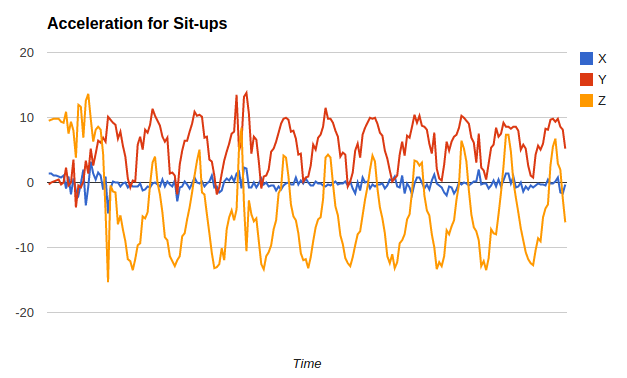
\includegraphics[width=0.80\textwidth]{images/Chart3.png}
	\caption{Acceleration in all axes during Sit-ups}
	\label{fig:acceleration2}
\end{figure}

For each exercise, we performed measurements with two test subjects and chose an axis with the highest response and a corresponding threshold. For several exercises, we combined the acceleration in two axes with the highest response, if their frequency was equivalent. An example can be seen on figure \ref{fig:acceleration2}.


\subsection{Pedometer}

To achieve the detection of steps some understanding of the walking movement is necessary. There are many parameters to describe the activity of walking such as distance, velocity, acceleration. We will use the acceleration to detect when a step is taken. We have chosen the accelerometer over GPS to allow people to walk inside the building as well, for example on their coffee break.
\\\\
When someone is walking there is some acceleration in their arms, waist, legs and feet. Acceleration of the feet is the most accurate but for the purposes of our project we will use the waist and leg acceleration since the pocket is the most obvious place for someone to have their phone and it is easy to carry that way.
\\\\
For measuring steps, we used the pedometer algorithm provided by \cite{1_berk_2014}. In short, the algorithm works by finding local minima and maxima in acceleration in the Z axis and comparing their difference to a threshold. The walking acceleration measured in one of our test sessions is presented on Figure \ref{fig:acceleration3}.

\begin{figure}[H]
	\centering
		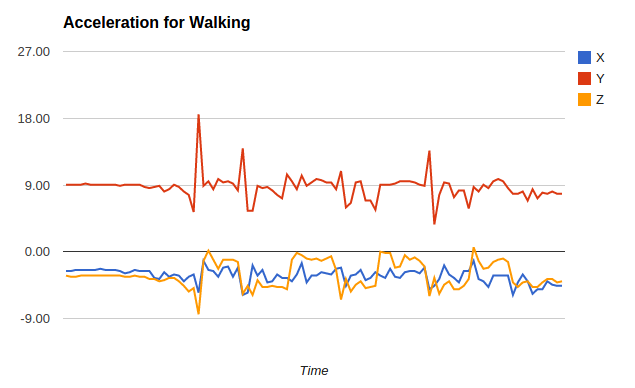
\includegraphics[width=0.80\textwidth]{images/Chart2.png}
	\caption{Acceleration of Walking}
	\label{fig:acceleration3}
\end{figure}


\subsection{Alternative approaches}

At this point it is important to explain why we chose not to get position out of the acceleration.
In order to achieve linear acceleration we need to compensate for gravity as follows:
\\\\
Linear acceleration = Accelerometer Data – Gravity
\\\\
Then we have to integrate it once to get velocity 
\\\\
$$v= \int a dt$$
\\\\
and then integrate it again to get position
\\\\
$$x= \int v dt$$
\\\\
However this method integrates noise and results to 20cm-8.5m of drift over a single second. So it is not suitable to measure our exercises since the error is much larger than the distance required to complete them.

\bibliography{sources}

\section{Challenges and Future Development}
We believe that the project has met all of its main requirements and even has some optional features. It can be noted however that the implemented features have not achieved sufficient depth to use this game for exercising over an extended period of time. Also there were some challenges on the way, which will also be discussed here.
\\\\
A nice technical improvement would be to expand the application so it can take into account the user’s physical measurements and suggest specific exercises based on the goals of the user. The great amount of personalization would require a lot of adaptations to the current game.
\\\\
Although the exercises are measured quite allright, it is still very much possible to improve the sensors. We have received a library to serve as an example, but that was not of significant help to the accuracy of the measurements. Extended research and testing would have to be done to exclude all possibilities of cheating from the exercises and really make them measure quality instead of merely quantity.
\\\\
We would have wanted to implement a heart rate sensor to check how well the user had done a timed exercise, but we didn't get to it. The code was there for a Java-based application, but not for PhoneGap, so it was too much trouble to rewrite the whole algorithm. This would be a very nice feature to add, because it takes away a lot of the cheating possibilities.
\\\\
The application is currently causing lag after a while, because it used up quite some memory. We are not really sure where this is coming from, and we would have liked to fix this when there was more time.
\\\\
Currently, when you zoom in or out the center of the screen shifts a couple of tiles, this might be a bit annoying. To fix this we would have to set a focus point. This was not a big priority however, so it has been skipped for this version.


\end{document}
